\chapter{Contexto Geológico}

A área de estudo enquadra-se geolologicamente no Rift Continental do Sudeste do Brasil(RCSB) sobre terrenos policíclicos referíveis ao sul do Cinturão de Dobramentos Ribeira, nomeada por \cite{Riccomini_1989} em seu trabalho, Sul do Cráton São Francisco e Sul da Faixa Brasília, como pode ser observado na Figura \ref{mapa_geologico}. Essa zona geológica é intulada por \cite{Almeida_Carneiro_1998} como Planalto Atlântico. Encontra-se nessa região retrabalhamento de ciclos orogênicos pretéritos e o conjunto lito1ógico está recortado por sistema de falhamentos transcorrentes (zonas de cisalhamento) orientados segundo a estruturação regional, direção ENE a EW, \cite{Hasui_Sadowski_1976}. As feições estruturais da região de estudo são fortemente influenciadas pelo Cinturão de Dobramentos Ribeira.

\begin{figure}[!ht]
\centering
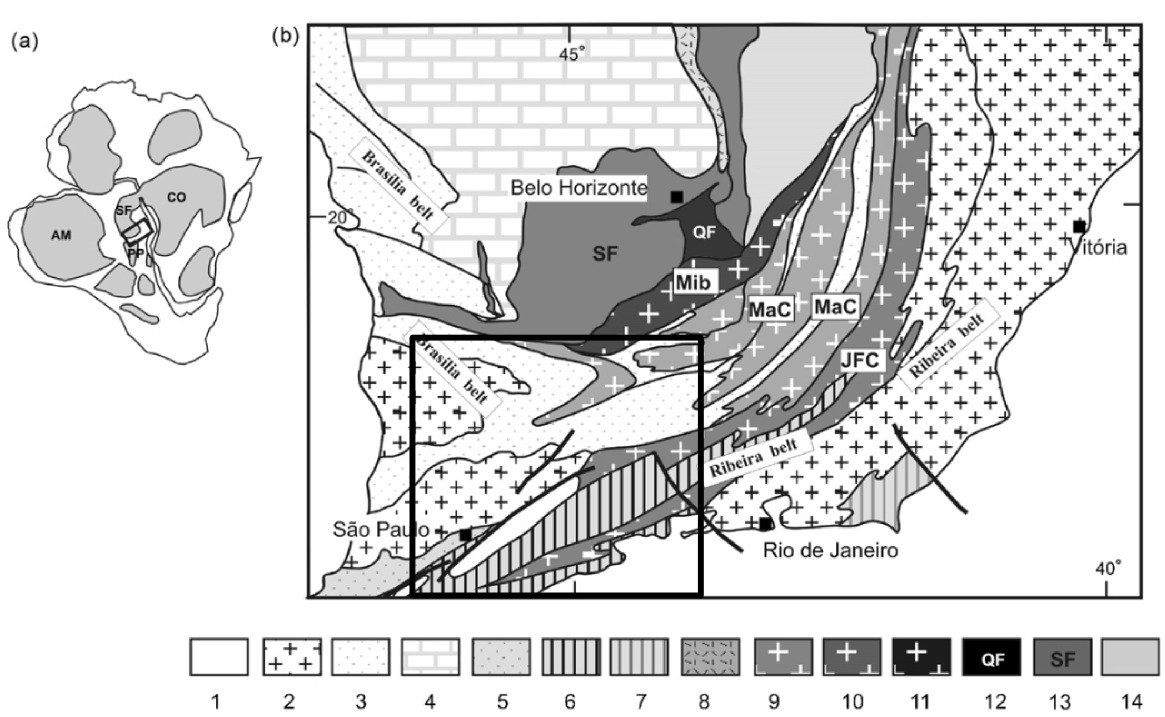
\includegraphics[scale=0.9]{mapa_geologico.png}
\caption{Mapa tectônico da Região do Sudeste do Brasil com a área de trabalho marcada pelo quadradro. Legenda: 1-Bacias do Paraná e do Rift Cenozóico. 2-Plutons alcalinos Cenozóicos/Cretácios. (3–4), 3-\textit{Nappe} Socorro(S)-Guaxupé(G); 4-Sistema \textit{Nappe} Andrelândia(ANS) e \textit{Nappe} Passos(P). Cráton São Francisco (5–7), 5-Embasamento, 6-Cobertura (Grupo Bambuí); 7-Cobertura (rochas metasedimentares autóctones e paraautóctones.;  Faixa Ribeira (8–15): 8-Domínio Andrelândia(AD) e equivalentes; 9-Domínio Juiz de Fora do Terreno Ocidental; 10-Terreno Paraíba do Sul; 11-Terrano Oriental incluindo  12-Arco Rio Negro; 13-Terreno Cabo Frio; 14-Terreno Embu; 15-Terreno Apiaí. CTB=Limite Tectônico Central e SFC=Craton São Francisco. A área sombreada cobrindo a parte sul da Faixa Brasília e a parte sudeste do Cráton São Francisco corresponde a uma zona de interferência onde a deformação e o metamorfismo da Faixa Ribeira se  sobressai na Faixa Brasília. Adaptado de \cite{trouw_new_2013}}
\label{mapa_geologico}
\end{figure} 

O sul da Faixa Brasilía foi descrito, \cite{pimentel_tectonic_2011},\cite{reno_situ_2012} e \cite{trouw_new_2013}, como resultado da colisão entre a margem passiva do paleocontinente São Francisco do leste com a margem ativa do bloco, ou paleocontinente, Paranapanema do lado oeste da sutura. Esta colisão produziu um empilhamento espesso de \textit{nappes} ao longo da sutura, como o Sistema de \textit{Nappe} Andrelândia(ANS). Dobras em bainha em grande escala e inúmeras dobras interropidas atestam a deformação dúctil intensa dentro das \textit{Nappes}. Lineamentos alongado, combinados com indicadores de cisalhamento mostram do norte para o sul a troca progressiva, cavalgando do topo para E-SE  na \textit{Nappe} Passos. A sutura desse cinturão é interpretada sendo localizada entre a \textit{Nappe} Socorro-Guaxupé e o Sistema \textit{Nappe} Andrelândia.

A Faixa Ribeira é composta por rochas metamórficas,migmatitos e granitóides relacionados ao Ciclo Orogenético Brasiliano, como citam \cite{kuhn_metamorphic_2004}, \cite{heilbron_evolution_2010} e \cite{valeriano_u_pb_2011}. Esta tendência estrutural regional pode ser observada na Figura \ref{mapa_geologico}. Segundo \cite{heilbron_evolution_2010} a Faixa Ribeira é composta por 4 terrenos tectônicos-estratigráficos separados por falhas de
empurrão ou por zonas de cisalhamento oblíquas transpressivas: (a) a margem retrabalhada do Cráton São Francisco definida como Terreno Ocidental; (b) O Terreno Paraíba do Sul-Embú que está cavalgando sobre o Terreno Ocidental;(c) O Terreno Oriental (Serra do Mar) que inclui o Arco Magmático Neoproterozóico, e (d) O Terreno Cabo Frio, que foi acrescionado depois, por votla de 520 M.a. Estes Terrenos estão demarcados na Figura \ref{mapa_geologico}. Estes são subdivididos em vários domínios, tais domínios são identificados devido ao seu contraste litológico, geoquímica isotópica e geocronologia, cita \cite{kuhn_metamorphic_2004}. A sutura entre o Terreno Ocidental e Oriental é uma zona de cisalhamento com mergulho-NW, também chamada de Limite Tectônico Central(CTB) por \cite{heilbron_evolution_2010} e \cite{trouw_new_2013}. Essa sutura pode ser mapeada continuamente por pelo menos 200 km entre a costa de São Paulo e a Serra do Órgãos, no estado do Rio de Janeiro. 

\cite{trouw_new_2013} sumariza as principais características dos terrenos que compõem a Faixa Ribera. O Terreno Ocidental é caraterizado por rochas do embasamento Paleoproterozóico a Arqueano, representado pelos Complexos Barbacena, Mantiqueira e Juiz de Fora, e por uma cobertura siliciclástica metamorfizada oriunda de uma margem passiva. Esta é chamada de Megassequência Deposicional Andrelândia. Já o Terreno ou Klippe Paraíba do Sul possui ortognaisses granodioríticos a graníticos do Complexo Quirino, de idade Paleoproterozóica e é coberta pelo Complexo Paraíba do Sul, gnaisses feldspáticos e pelíticos, com intercalações de mármores dolomíticos. O Terreno Oriental alojaortognaisses tonalíticos a granodioríticos pertencentes ao Complexo Rio Negro, bem como metassedimentos Neoproterozóicos, ricos em intercalações carbonáticas e rochas metabásicas. A Colisão deste terrenos acarretou na geração de vários tipos de rochas granitóides sin-colisionais: leucogranitos, charnockitos, granitos porfiróides e bitotita granitos. Por fim, o Terreno Cabo Frio engloba ortognaisses Paleoproterozóicos do Complexo Quirino e uma sucessão metassedimentar com gnaisses pelíticos com cianita, sillimanita e granada, metabasitos e rochas calcissilicáticas. 

Outras grandes estruturas presentes na região da Faixa Ribeira são as bacias sedimentares que seguem a região é Rift Continental do Sudeste do Brasil (RCSB), como pode ser visto na Figura \ref{mapa_estacoes_geologico}. \cite{Riccomini_1989} apresenta o RCSB como uma depressão alongada e deprimida com mais de 900 km de comprimento entre os estados Paraná e Rio de Janeiro. Este Rift possui uma idade paleógena e segue a linha de costa atual, alcançando o Oceano Atlântico em seu segmento ocidental e na sua Terminação nordeste. Inúmeros corpos alcalinos de idade cretácica a paleogênica ocorrem ao longo das bordas desse sistema de Rifts. A área em estudo engloba o segmento central do RCSB. Este possui as bacias sedimentares de São Paulo, Taubaté, Resende e Volta Redonda, como pode-se observar nas áreas com tonalidades em amarelo na Figura \ref{mapa_estacoes_geologico}. 

\begin{figure}[!ht]
\centering
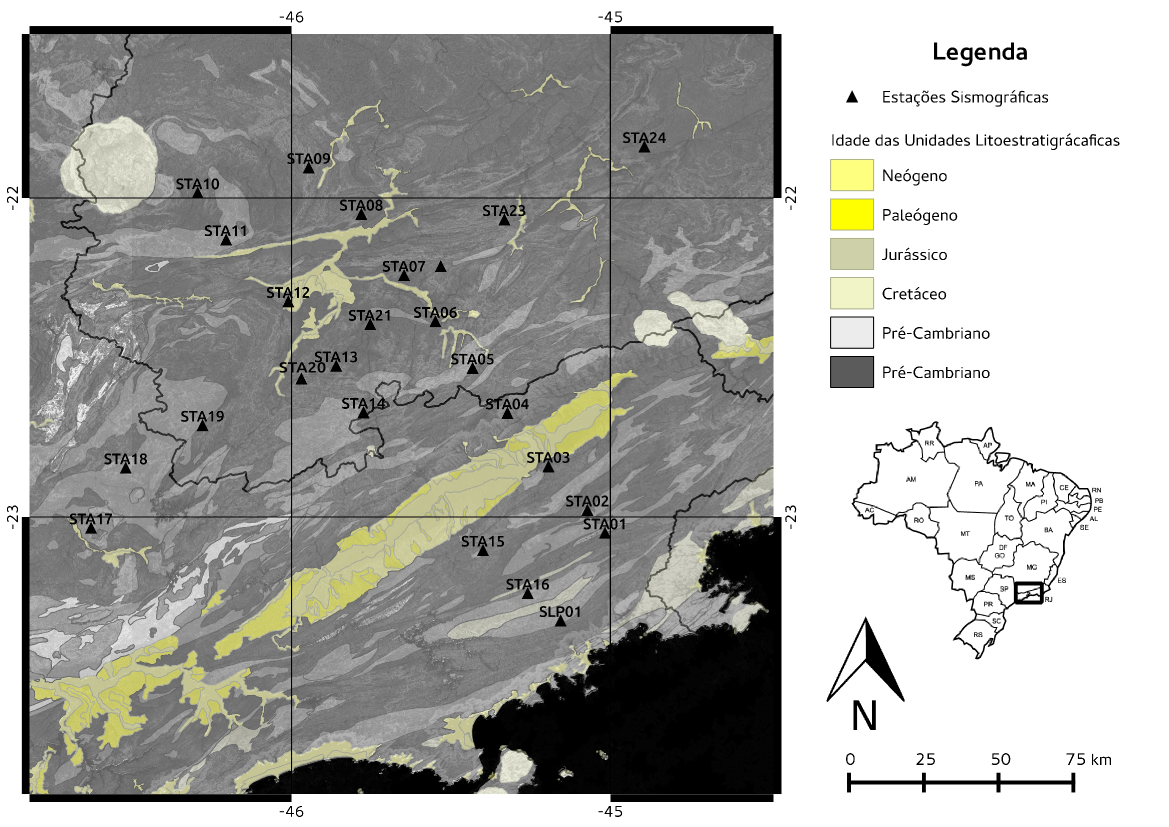
\includegraphics[scale=0.5]{mapa_estacoes_geologico.png}
\caption{Mapa de localização das Estações Sismográficas na região com o mapa simplificado das unidades litológicas da folha SF-23 Rio de Janeiro.}
\label{mapa_estacoes_geologico}
\end{figure}

